\chapter{Project Plan}

% \instructions{
%     Describe the project plan as covered in the SEP2 module. A project plan typically consists of the following topics:
    
%     \begin{itemize}
%         \item Processes, meetings and roles
%         \item Phases, iterations and milestones
%         \item A \textbf{rough} list of things to be done (work items)
%         \item Risk management
%         \item Planning Tools (issue tracker, time tracker, ...)
%     \end{itemize}
    
%     You should \textbf{\underline{not}} describe your \textbf{technical solution} in this chapter. It is all about organizing your project.
% }

\section{Processes}
For the long-term planning we use RUP (\ref{phases}).
For the short-term planning we use Scrum.
The Scrum roles and other assignments are described in \ref{roles}.
The Scrum Events (Sprint Planning, Sprint Review, ...) are declared in \ref{meetings}.
How we implement the Scrum artifacts is defined in \ref{scrum}.

\subsection{Git Workflow}
\label{git-workflow}
When working on source code a new branch must be created.
Before merging into the main branch the source should be approved by someone else from our team.
The same also applies to Kubernetes configuration files.
Except the changes were produce in a pair programming session.
Working on the master branch directly is only allowed when the documentation is updated.

\subsection{Scrum}
\label{scrum}
For the short term planning iteration we use the Scrum method.
In the following we describe how we want to implement the Scrum process using GitLab.

\begin{table}
    \centering
    \caption{Scrum process elements}
    \label{tab:scrum-elements}
    \begin{tabular*}{\textwidth}{ p{5cm} | p{9cm} }
        \textbf{Scrum} & \textbf{GitLab} \\ 
        \hline
        \textbf{Epic:} & Label with format Epic:xxx \\
        \textbf{User Story / Feature:} & Numbered issues starting with FR:xx (for Functional Requirements), tagged with User Story label plus MVP label if appropriate \\
        \textbf{Work Item:} & Issue linked to the User Story issue \\
        \textbf{Prioritization:} & Prioritized labels: low, medium, important, critical \\
        \textbf{Story Points:} & Label with format xx\$ \\
        \textbf{Scrum Board:} & Issue Board \\
    \end{tabular*}
\end{table}

\noindent To build our Scrum Board the following labels are required:

\begin{itemize}
\item ToDo - no work done yet
\item WIP - work in Progress
\item Done - done, but do not close (yet)
\end{itemize}

\noindent We manage the status of Work Items with the above labels. Work Item issues should not be closed during an ongoing sprint, rather the label \textsl{Done} should be assigned (and \textsl{WIP} removed). Once the sprint is complete, all Work Item issues from that particular sprints are closed at once. The reason for this approach is have an overview per sprint what we have already done. We created a Board using the above labels to monitor the progress.

\noindent To build our Story map the following labels are required \footnote{\url{https://gitlab.ost.ch/SEProj/2022-FS/g03-kubewatch/kubewatch/-/boards/935}}:

\begin{itemize}
\item Epic:xxx
\item User Story
\item Product Backlog
\item Operational
\end{itemize}

\section{Roles}
\label{roles}

\begin{table}[h]
    \centering
    \caption{Project roles}
    \label{tab:project-roles}
    \begin{tabular}{l|l}
        \textbf{Role} & \textbf{Person}\\ \hline
        \textbf{Session Chair:} & Changes every week \\
        \textbf{Product Owner (PO):} & The whole team \\
        \textbf{Developer:} & Benjamin Plattner, Olivier Lischer, Pascal Lehmann\\
        \textbf{Infrastructure \& Network:} & Jan Untersander, Petra Heeb \\
    \end{tabular}
\end{table}

\noindent The classification in \textsl{Developer} and \textsl{Network} shows only the primary strengths.
Members of the \textsl{Developer} group sometimes also work on the network part and vice versa.


\section{Meetings}
\label{meetings}
We have two weekly meetings: \newline
The first is an internal team meeting every Monday morning is used to implement:
\begin{itemize}
  \item Sprint Planning
  \item Sprint Retrospective 
\end{itemize}

\noindent The second meeting takes place every Tuesday noon with our advisor Laurent Metzger.
In this meeting the \textsl{Sprint Review} is done.
\newline
\noindent The \textsl{Daily Scrum} take places during the week at lunch or during breaks.
One Sprint lasts two weeks.


\section{Phases, iterations and milestones}
\label{phases}
In our project we work with the four project phases which are defined also in the RUD model which we used for our rough project plan. The four phases are:
\begin{itemize}
    \item Inception
    \item Elaboration
    \item Construction
    \item Transition
\end{itemize}

\subsection{Inception}
The first phase is the \textit{Inception} phase. In this phase we start the new project and  define the following items to plan our project:
\begin{itemize}
    \item Approximate vision
    \item Defining the scope
    \item Rough estimates of efforts
\end{itemize}

\subsection{Elaboration}
The second phase is called \textit{Elaboration}. This phase is used to start the practical part of the project and the goal of this phase is to eliminate potential risks, sometimes using prototypes. There are a few parts we need to handle during this phase:
\begin{itemize}
    \item Identification of most requirements
    \item Iterative implementation of the core architecture
    \item Resolution of high risks
    \item More realistic estimates for efforts
\end{itemize}

\subsection{Construction}
The third and biggest phase is the \textit{Construction} phase. In this phase the team needs to implement the features defined in the project to achieve the product goal. All identified risks should be eliminated by that time or mitigations should be in place to control the risks. The main goal is to have a product ready that can be deployed.
The contents of this phase are:
\begin{itemize}
    \item Iterative implementation of functionality
    \item Resolution of lower risks
    \item Preparation for deployment
\end{itemize}

\subsection{Transition}
The last project phase is called the \textit{Transition} phase during which the project is tested in the whole environment and the project is finished.
The basic elements of this final phase are:
\begin{itemize}
    \item Beta Tests
    \item Deployment
    \item Tie up any loose ends
\end{itemize}

\section{Project Plan}
\subsection{RUD - Rational Unified Process}
To define a rough project plan we use the RUD model which is defined in weekly steps. \newline

% \begin{figure}[h]
    % \centering
    % \caption{\label{fig:project-plan}KubeWatch project plan}
    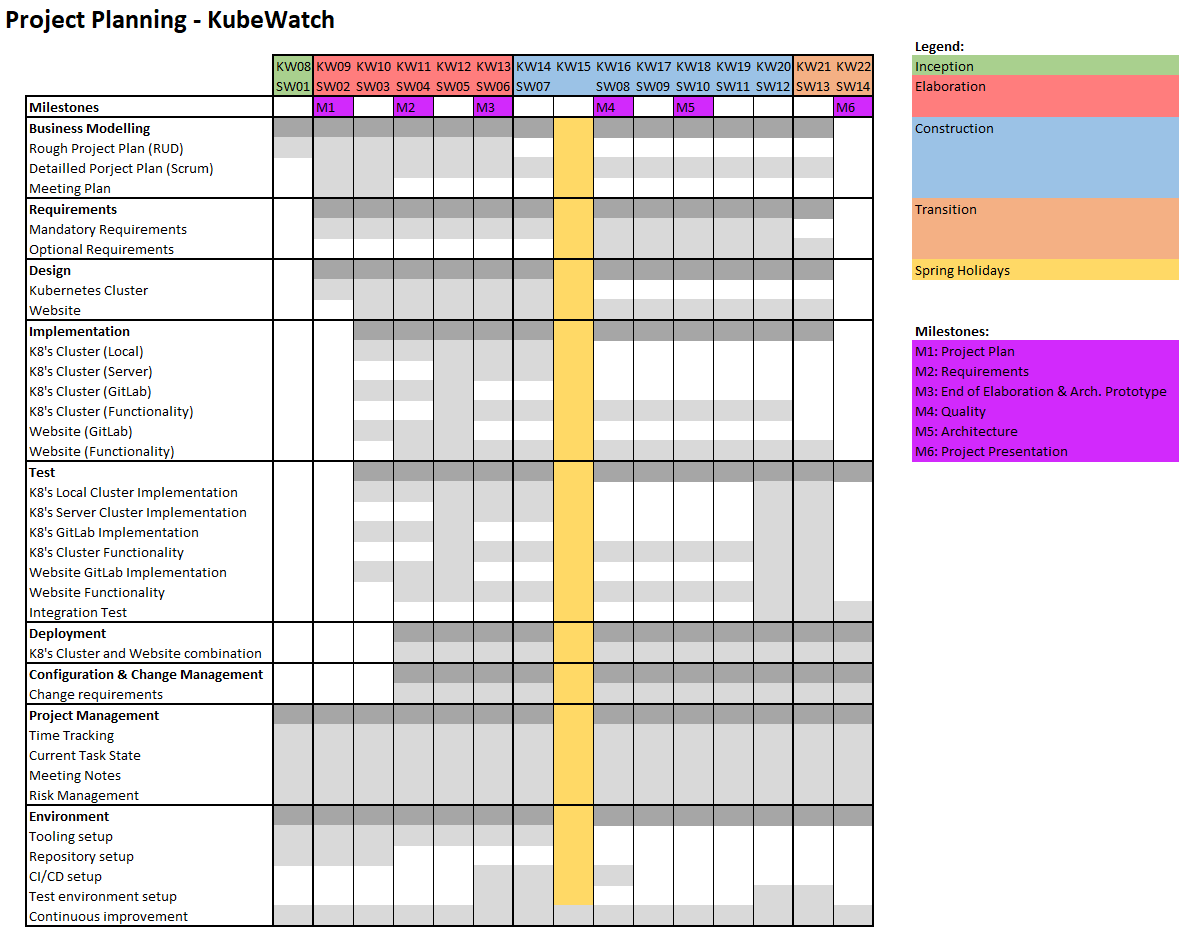
\includegraphics[width=\textwidth]{resources/project-plan-RUD.png}
% \end{figure}

The project plan can be found in the project's repository\footnote{\url{https://gitlab.ost.ch/SEProj/2022-FS/g03-kubewatch/kubewatch/-/tree/main/Documentation/src/03_project-documentation}}.

\section{Planning Tools}
For planning our work, issue handling and time tracking we use GitLab issues, merge requests and the built-in time tracking functionality.

\section{Risk Management}

As part of a continuing risk management analysis, we use a risk matrix to estimate the impact of the identified risks.\newline
We use a spreadsheet to quantify the risks and to create the resulting figure. The current risk matrix can be seen in figure \ref{fig:risk-matrix}. It presents an overview of the categorisation of the identified risks. Table \ref{tab:risk-classification} presents a detailed description of all identified risks.

\begin{figure}[h!]
    \centering
    \caption{KubeWatch Risk Matrix}
    \label{fig:risk-matrix}
    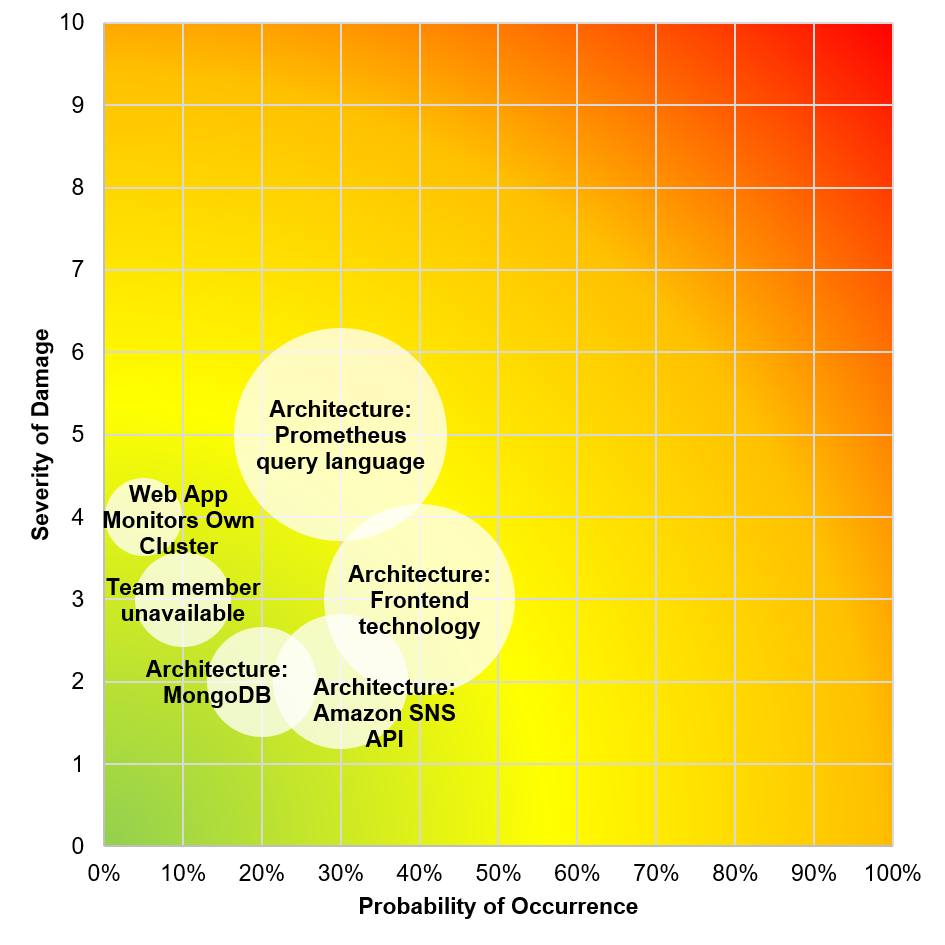
\includegraphics[width=11cm]{resources/risk_matrix.png}
\end{figure}

\subsection{Risk Methodology}
We use a risk weighted approach to estimate the impact of a new risk. The impact is calculated as the product of the 'severity of the damage', which is a category of scale 1 to 10, and the 'probability of occurrence'. To better gauge the severity of damage, we use a relativistic approach where we compare existing risks with new risks and decide on the relative impact of one risk versus others.

\subsection{Risk Review Process}
The identification and analysis of new risks happen continuously, but at least once every new sprint. There, the team discusses potential new risks and one team member is then assigned to update the documentation accordingly.

The table \ref{tab:risk-review} lists all risk reviews.

\begin{table}[h!]
\centering
  \caption{\label{tab:risk-review}Risk Reviews and Changelog}
  \begin{tabular}{ | p{2cm} | p{11cm} | } \hline
    \textbf{Date} & \textbf{Changes} \\ \hline
    03.03.22 & Created initial analysis. \\ \hline
    14.03.22 & Risks reviewed. Added risk 'Web App Monitors Own Cluster'. \\ \hline
    01.04.22 & Risks reviewed and metrics updated, mainly because of additional mitigation measures. Eliminated 'Unknown API', added 'Simple Notification Service API'. \\ \hline
  \end{tabular}
\end{table}

\begin{longtable}[h!]{p{2.2cm} | p{4cm} | p{4cm} | p{1.5cm} | p{1.5cm} | p{1.5cm}}
    \textbf{Risk Name} & \textbf{Risk Description} & \textbf{Mitigation} & \textbf{Probability of Occurrence} & \textbf{Severity of Damage (0-10)} & \textbf{Weighted Damage} \\ 
    \endhead
    \caption{\label{tab:risk-classification}Classification of identified risks}
    \endlastfoot
    \hline
        Kubernetes Cluster
            & The deployment and setup of the Kubernetes Cluster has only been performed by Petra and Jan as part of their Cloud Infrastructure class. It may take a long time to fully configure the desired setup.
            & With the help of the INS we can leverage their expertise in setting up K8s clusters and apply default configurations.
            & \multicolumn{1}{c}{Eliminated} \\ \hline
        Unknown API for MVP
            & The API to extract data points from the K8s cluster is new to us. There are libraries like Prometheus which can collect such data, but we do not have much experience using it.
            & We have tested the APIs as part of the prototype design and we were able to fully connect all necessary APIs for our MVP. Hence this risk is now mitigated. There is an additional risk for a potential extension of functionality, which is described separately.
            & \multicolumn{1}{c}{Eliminated} \\ \hline
        Accessing K8s Cluster 
            & To access the K8s Cluster that is set up in the INS, we need to define the best way for everyone to work on the Cluster and subsequently the Web API.
            & The INS has different options to access the cluster, but we have not yet been able to test it. However, we deployed the web application locally on a K8s cluster which workes just fine. Therefore, the likelihood of this risk impacting the project is significantly reduced.
            & 10\% & 7 & 0.7 \\ \hline
        Unknown Development Environment
            & To run a Web Server on a K8s Cluster is new for us and may come with certain obstacles which would not appear in a local development environment. However, the tech stack we are planning on using is well-known to us.
            & Each of the team members tested the local development environment and it works. The development environment on the INS Cluster is not fully tested, this should be done as soon as possible. But with this step the risk for the development environment is mostly mitigated.
            & 20\% & 5 & 1.0 \\ \hline
        Scrum Methodology 
            & We are applying an Agile approach for the development of this project. The Scrum framework is best suited for us as it has clear guidelines. However, we do not have much experience in running Scrum methodologies.
            & The Software Engineering Project module, which we attend in parallel, is designed to support us in learning and applying Scrum. During the last weeks we got some regularity in how to use agile methodologies and it works really good until now. There is a small residual risk because we need more practice in implementing and applying Scrum to be most beneficial for our needs.
            & 10\% & 1 & 0.1 \\ \hline
        New Architecture 
            & Designing a new architecture for a project for which we have no prior experience is always a risk that something gets overlooked.
            & The architecture for our desired final state of the project is not overly complex. Also, we have experience with most of the individual components that we intend to use, just not in combining them in the desired setup. In the last week we create an architecture overview which helps us to manage each component and understand the combinations. While this process reduced the risk significantly, there is still a probability that we did not combine the components correctly, or we need to change the architecture at a later which is quite costly for the project.
            & 30\% & 8 & 2.4 \\ \hline
        Team member unavailable
            & One or more team members may become unavailable for the project due to illness, accident or other personal reasons. In this case, the workload must be spread across fewer members, which has an impact on the timeline. Also, information may get lost that was only available to that person.
            & Information sharing across team members is important. We formed two sub-groups (Network and Web development) where information is shared, and we train each other during the weekly meetings on important developments. In addition, we maintain a practice of documenting code and other implementation specific details in a shared repository. Thanks to an agile approach, change in timelines only impact the number of features available in the final product, rather than posing a threat to the success of the overall project.
            & 10\% & 3 & 0.3 \\ \hline
        Web App Monitors Own Cluster
            & The Web Application that monitors the Kubernetes Cluster runs on the same Cluster which it monitors. This may become a risk if the Cluster or Node where the app runs goes down unexpectedly so that a notification cannot be sent before the shutdown.
            & We are aware of this issue and constantly monitor the Cluster while development is ongoing. Once in production, the app should then reside on a separate Cluster. Development happens on a local and smaller version of Kubernetes (Minikube), which lowers this risk and impact drastically.
            & 5\% & 4 & 0.2 \\ \hline
        Amazon Simple Notification Service API
            & As a potential extension to the basic push notification on the Web Application itself, we intend to add the ability to notify a user through email. The Amazon Simple Notification Service (SNS) API would provide this feature in a way that is easy to setup and configure.
            & We have not yet been able to test this API as we are still in the elaboration phase and will soon be focused on developing the MVP which does not yet include this feature. There is a risk that this API does not work as expected, and we have not yet requested an account for it. The alternative would be to set up an email service through an established email provider, which we know would work. However, the latter option would be more cumbersome to manage.
            & 40\% & 2 & 0.8 \\ \hline
\end{longtable}


\section{Description of our Epics}

As we work with Epics and User Stories, we briefly describe the Epics here to put them into the context of KubeWatch's use case.

\subsection{User Management}
When KubeWatch is used by different K8s cluster users who are not part of the same team, the user management allows KubeWatch to have a login site where users need to authenticate themselves. In addition, a user might join a user group where dashboards and thresholds can be shared. The user management simplifies the authentication and access to content. This Epic is not part of the MVP.

\subsection{Data Visualisation}
A KubeWatch user's main goal is to monitor the performance of a K8s cluster, its nodes and other K8s resources. This is achieved by visualising different metrics in different charts. These charts will be displayed in different windows in the web app. The MVP contains a static dashboard whose only purpose is to demonstrate the capabilities and give a first impression of the tool. Subsequent user stories provide dynamically creatable charts with automatic updating data, along with a customisable dashboard. If the user management is implemented, each user group can also create and save their own dashboards.

\subsection{Notification}
A key feature of KubeWatch is to notify the K8s user if a cluster, node or other K8s resource is in a critical state, for example has a too high CPU utilisation, is out of memory, or went down. The notification feature enables this by alerting a K8s user in the KubeWatch dashboard, via email or other notification channels. To trigger a notification, the K8s user needs to define certain thresholds, like CPU usage or memory consumption, above which the user would like to get an alert. The MVP will feature simple display notifications which the user can dismiss, along with accessing the notification history. Subsequent user stories will then feature alerts based on live data, as well as extending the notification format to email, SMS and potentially other services.

\subsection{Cluster Visualisation}
When working with K8s clusters for the first time, it is helpful to quickly get an overview of how certain elements of the cluster are working together. Cluster Visualisation provides the K8s user a simple dashboard where basic, but relevant information is quickly visible. This visualisation shows the different types of nodes (master, worker) and different K8s resources running or belonging to these nodes, like deployments, replicaSets and pods. This feature is not part of the MVP. A potential first release would display static data to give the user a taste of the capabilities, whereas a subsequent release would display live data. 

\subsection{Cluster Configuration}
It may be convenient for a K8s user to do simple configurations of K8s clusters through the KubeWatch tool. The Cluster Configuration enables this feature by providing access to clusters like the Kubernetes Dashboard, but in a simpler manner. This feature is a potential extension and is not a key feature of KubeWatch at this point. Therefore, it is not part of the MVP.

\subsection{Operational}
To enable all the planned features of KubeWatch, there are many backend configurations and setups required. This includes, for example, automated deployment of feature releases, creating and managing a database to store KubeWatch data, like user-defined thresholds, or other tools to get the development team organised. Everything that is not part of a user story is therefore captured in Operational. The concept of an MVP does not apply here, as many of the items in this Epic are continuous (like time tracking), and are only indirectly relevant to every major release.

\section{Personas}

The purpose of using KubeWatch is to monitor the performance of a Kubernetes Clusters. A typical K8s user is a rather technically adept person who usually has some Computer Science background or is at least very familiar with K8s and containerisation. This user has a specific need to monitor the health of their cluster and is assumed to be capable of configuring KubeWatch themself. Hence, as we intend to create this tool with only one specific user in mind, for which we have a clear understanding of their requirements, we decided to omit the creation of specific personas for this project.

